\UseRawInputEncoding
\documentclass[12pt]{article}
\title{ECE 102 Homework 5}
\usepackage{subcaption}
\author{Lawrence Liu}
\usepackage{graphicx}
\usepackage{amsmath}
\usepackage[scr]{rsfso}

\newcommand{\Laplace}{\mathscr{L}}
\setlength{\parskip}{\baselineskip}%
\setlength{\parindent}{0pt}%
\usepackage{xcolor}
\usepackage{listings}
\definecolor{backcolour}{rgb}{0.95,0.95,0.92}

\lstdefinestyle{mystyle}{
    backgroundcolor=\color{backcolour}}
\lstset{style=mystyle}

\begin{document}
\maketitle
\section{Problem 1}
\subsection*{(a)}
We have that 
$$x(t)=\sum_{k=-\infty}^{+\infty}a_ke^{jk\omega_0t}$$
Therefore we have
\begin{align*}
y(t)&=x(2t-3)+4\frac{d^2x(t)}{dt^2}\\
&=\sum_{k=-\infty}^{+\infty}a_ke^{jk\omega_0(2t-3)}+4\frac{d^2}{dt^2}\sum_{k=-\infty}^{+\infty}a_ke^{jk\omega_0t}\\
&=\sum_{k=-\infty}^{+\infty}a_ke^{-3jk\omega_0}e^{j2k\omega_0t}+4\sum_{k=-\infty}^{+\infty}a_k\frac{d^2}{dt^2}e^{jk\omega_0t}\\
&=\sum_{k=-\infty}^{+\infty}a_ke^{-3jk\omega_0}e^{j2k\omega_0t}-4\sum_{k=-\infty}^{+\infty}a_kk^2\omega_0^2 e^{jk\omega_0t}
\end{align*}
$$b_k=\boxed{\begin{cases}
-4a_k k^2\omega_0^2 & \text{if k is odd}\\
a_{k/2}e^{\frac{-3jk\omega_0}{2}}-4a_k k^2\omega_0^2& \text{if k is even}
\end{cases}
}
$$
\subsection*{(b)}
if 
$$x(t)\to a_k$$
we have
\begin{align*}
x(t+1)&\to a_ke^{jk\omega_0}\\
e^{j\omega_0t}x(t+1)&\to a_{k-1}e^{j(k-1)\omega_0}\\
\int_{-\infty}^{t}e^{-j\omega_0t}x(t+1)&\to\frac{1}{jk\omega_0} a_{k-1}e^{j(k-1)\omega_0}\\
\int_{-\infty}^{t+2\alpha}e^{-j\omega_0t}x(t+1)&\to\frac{1}{jk\omega_0} a_{k-1}e^{j(k-1)\omega_0}e^{2jk\omega_0\alpha}
\end{align*}

Thus we get
$$b_k=\boxed{\frac{1}{jk\omega_0} a_{k-1}e^{j(k-1)\omega_0}e^{2jk\omega_0\alpha}}$$
\subsection*{(c)}
\begin{align*}
y(t)=\frac{dx^3(t)}{dt}\\
=3x^2(t)\frac{dx(t)}{dt}
\end{align*}
Thus we get that
\begin{align*}
b_k&=3\int_{T_0}x^2(t)x'(t)e^{-jk\omega_0 t}
\end{align*}
Since 
$$x(t)=\sum_{k=-\infty}^{+\infty}a_ke^{jk\omega_0t}$$
$$x'(t)=\sum_{k=-\infty}^{+\infty}jk\omega_0a_ke^{jk\omega_0t}$$
Thus we get
$$b_k=\boxed{3\sum_{n+m+p=k}a_na_mjp\omega_0a_p}$$
\section*{Problem 2}
\subsection*{(a)}
for $k\neq 0$
\begin{align*}
a_k&=\frac{1}{6}\int_{-3}^{3}x(t)e^{-jk\frac{2\pi}{6}t}dt\\
&=\frac{1}{6}\left(\int_{-2}^{-1}(t+2)e^{-jk\frac{2\pi}{6}t}dt+\int_{-1}^{1}e^{-jk\frac{2\pi}{6}t}dt+\int_{1}^{2}(-t-2)e^{-jk\frac{2\pi}{6}t}dt\right)\\
&=\frac{3(\cos(\frac{\pi k}{3})-\cos(\frac{2\pi k}{3}))}{\pi^2k^2}
\end{align*}

for $k=0$
$$a_0=\frac{1}{2}$$
\subsection*{(b)}
\begin{center}
\begin{figure}[h]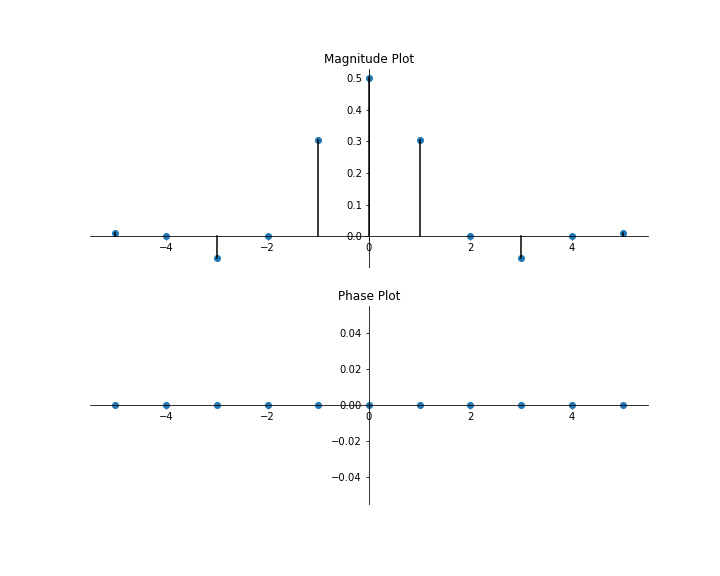
\includegraphics[width=10cm]{fig1}
\end{figure}
\end{center}
\pagebreak
\subsection*{(c)}
$$x(t)=r(t+2)-r(t+1)-r(t-1)+r(t-2)$$
$$x(t-2)=r(t)-r(t-1)-r(t-3)+r(t-4)$$
$$e^{-2s}X(s)=\frac{1}{s^2}-\frac{e^{-s}}{s^2}-\frac{e^{-3s}}{s^2}+\frac{e^{-4s}}{s^2}$$
$$X(s)=\frac{e^{2s}-e^s-e^{-s}+e^{-2s}}{s^2}$$
$$a_k=\frac{1}{6}\left.X(s)\right|_{s=\frac{jk\pi}{3}}=\frac{3(\cos(\frac{\pi k}{3})-\cos(\frac{2\pi k}{3}))}{\pi^2k^2}$$
\subsection*{(d)}
\begin{align*}
x(t)&=\frac{1}{2}+\sum_{k=1}^{\infty}a_ke^{k\Omega_0ti}+a_{-k}e^{-k\Omega_0ti}\\
&=\frac{1}{2}+\sum_{k=1}^{\infty}a_k(e^{k\Omega_0ti}+e^{-k\Omega_0ti})\\
&=\frac{1}{2}+2\sum_{k=1}^{\infty}a_k\cos(k\Omega_0t)
\end{align*}

Thus we get
$$a_k=\frac{3(\cos(\frac{\pi k}{3})-\cos(\frac{2\pi k}{3}))}{\pi^2k^2}$$
and 
$$b_k=0$$
\section*{Problem 3}
\subsection*{(a)}
$$x(t)=\sum_{k=-\infty}^{\infty}e^{-2jk\pi}e^{2jk\pi t}$$
thus we get
\begin{align*}
y(t)&=\sum_{k=-\infty}^{\infty}e^{-2jk\pi}H(jk2\pi)e^{2jk\pi t}\\
&=\sum_{k=-\infty}^{\infty}e^{-2jk\pi}\frac{1}{jk2\pi+4}e^{2jk\pi t}\\
&=\sum_{k=-\infty}^{\infty}\frac{e^{2jk\pi(t-1)}}{jk2\pi+4}
\end{align*}
\subsection*{(b)}
$$x(t)=\sum_{k=-\infty}^{\infty}\left(e^{-2jk\pi}-e^{-jk\pi}\right)e^{jk\pi t}$$
thus we get
\begin{align*}
y(t)&=\sum_{k=-\infty}^{\infty}\left(e^{-2jk\pi}-e^{-jkpi}\right)H(jk\pi)e^{jk\pi t}\\
&=\sum_{k=-\infty}^{\infty}\left(e^{-2jk\pi}-e^{-jkpi}\right)\frac{1}{jk\pi+4}e^{jk\pi t}\\
&=\sum_{k=-\infty}^{\infty}\frac{e^{jk\pi(t-2)}-e^{jk\pi(t-1)}}{jk\pi+4}
\end{align*}
\section*{Problem 4}
\subsection*{(a)}
From conditions (i,ii,iv,v) we get that $x(t)$ must be of the 
$$x(t)=2X_1\cos(t\frac{\pi}{3})+X_2e^{t\frac{2\pi}{3}}+X_{-2}e^{-t\frac{2\pi}{3}}$$
From condition iii we get
\begin{align*}
x(t)&=-x(t-3)\\
2X_1\cos(t\frac{\pi}{3})+X_2e^{t\frac{2\pi}{3}}+X_{-2}e^{-t\frac{2\pi}{3}}&=-2X_1\cos((t-3)\frac{\pi}{3})-X_2e^{(t-3)\frac{2\pi}{3}}-X_{-2}e^{-(t-3)\frac{2\pi}{3}}\\
&=-2X_1\left(\cos(t)\cos(\pi)+\sin(t)\sin(\pi)\right)-X_2e^{t\frac{2\pi}{3}}-X_{-2}e^{-t\frac{2\pi}{3}}\\
&=2X_1\cos(t)-X_2e^{t\frac{2\pi}{3}}-X_{-2}e^{-t\frac{2\pi}{3}}
\end{align*}

Since this must hold for all $t$ we get that $X_2=0$ and $X_{-2}=0$
Similarly from condition (vi) we get that $X_1=\frac{1}{2}$, thus
$$x(t)=\cos(\frac{\pi t}{3})$$
\subsection*{(b)}
\subsubsection*{(i)}
$x(t)$ is not real
\subsubsection*{(ii)}
$x(t)$ is not even
\subsubsection*{(iii)}
Since $x(t)$ is odd, its derivative is odd.
\section*{Problem 5}
We can find the coefficients of the Fourier series by calculating the Laplace transform of $x(t)$.

For $x_1(t)=u(t)-u(t-1)$

$$X(s)=\frac{1-e^{-s}}{s}$$
thus
$$a_k=\frac{1}{2}\left.X(s)\right|_{s=jk\pi}=\frac{1-e^{-jk\pi}}{2jk\pi}$$
Therefore the plot of the magnitudes of $x_1(t)$ is
\begin{center}
\begin{figure}[h]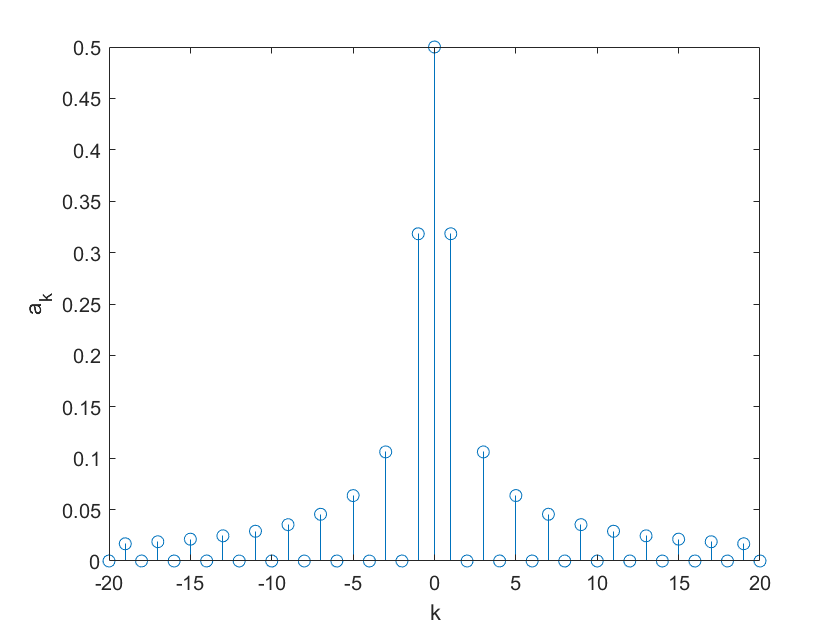
\includegraphics[width=10cm]{fig2}
\end{figure}
\end{center}

For $x_1(t)=r(t)-2r(t-1)+r(t-2)$

$$X(s)=\frac{1-2e^{-s}+e^{-2s}}{s^2}$$
thus
$$a_k=\frac{1}{2}\left.X(s)\right|_{s=jk\pi}=-\frac{1}{2}\frac{1-2e^{-jk\pi}+e^{-2jk\pi}}{k^2\pi^2}$$
Therefore the plot of the magnitudes of $x_2(t)$ is
\begin{center}
\begin{figure}[h]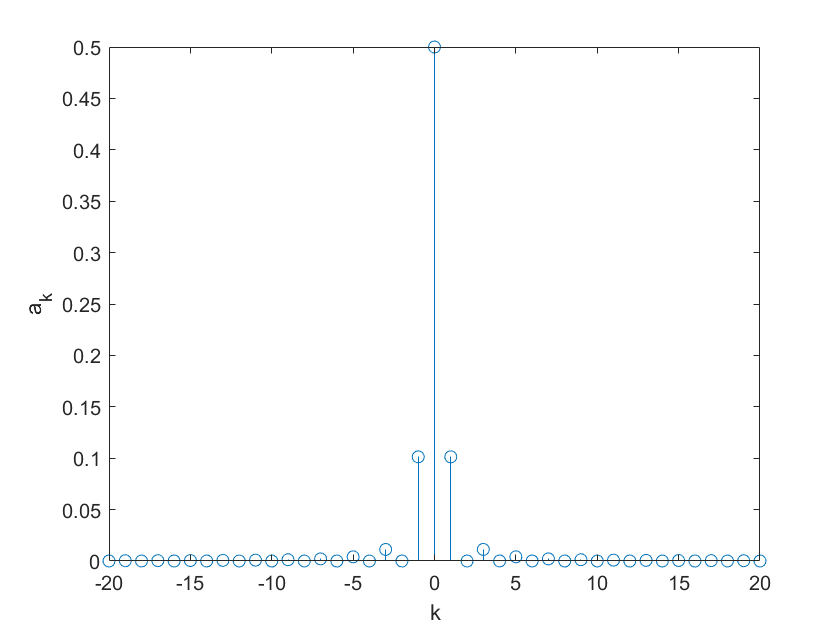
\includegraphics[width=10cm]{fig3}
\end{figure}
\end{center}
\pagebreak
The Fourier series coefficents for $x_2(t)$ decayed faster than those for $x_1(t)$ as $|k|$ increased. This means that $x_2(t)$ is "smoother" since for of the signals is distributed in the lower frequencies
\end{document}
